% https://texample.net/tikz/examples/islamic-art/
% Author: Amir Etemadi
% Drawing: Modernized Islamic Art
% October 15, 2011
\documentclass{minimal}
\usepackage{tikz}
\usepackage{calc}
\usetikzlibrary{spy}
%The base shape for this drawing is constructed by line segments
% of two lengths: \longd & \shortd
\newlength\longd
\newlength\shortd
\setlength{\longd}{0.5cm}
\setlength{\shortd}{0.2cm}

% The base shape is created by defining a new command.
%Polar coordination is used to find the important vertices.
% Some of the corners are rounded and others are sharp.
% The base shape is shaded using \shade draw command.
% The new command has three parameters which define
%the inner color, the outer color, and the border color.
\newcommand{\myshape}[3]{
   \shadedraw[inner color=#1,outer color=#2, draw=#3 ]
   (O)[rounded corners=4pt] --
   ++(90:\longd)[sharp corners] --
   ++(210:\shortd)[rounded corners=4pt] --
   ++(150:\shortd) --
   ++(30:\longd)--
   ++(330:\longd)[sharp corners] --
   ++(210:\shortd)[rounded corners=4pt] --
   ++(150:\shortd)--
   ++(-90:\longd) --
   ++(90-120:\longd) [sharp corners]--
   ++(210-120:\shortd)[rounded corners=4pt] --
   ++(150-120:\shortd)--
   ++(30-120:\longd) --
   ++(330-120:\longd)[sharp corners] --
   ++(210-120:\shortd)[rounded corners=4pt]--
   ++(150-120:\shortd)--
   ++(-90-120:\longd) --
   ++(90-240:\longd) [sharp corners]--
   ++(210-240:\shortd)[rounded corners=4pt] --
   ++(150-240:\shortd) --
   ++(30-240:\longd) --
   ++(330-240:\longd)[sharp corners] --
   ++(210-240:\shortd)[rounded corners=4pt] --
   ++(150-240:\shortd)-- cycle;
}
\begin{document}
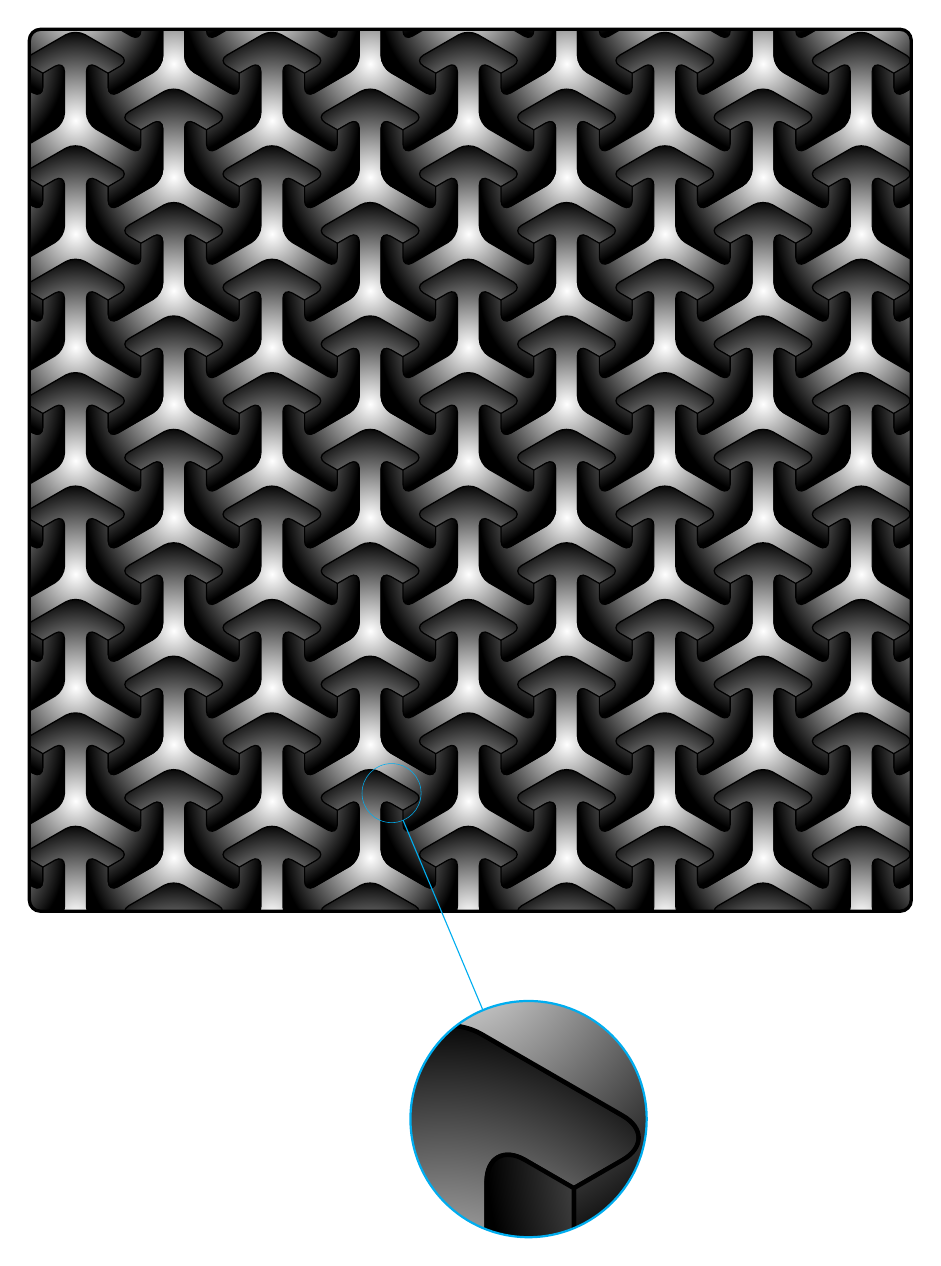
\begin{tikzpicture}[scale=1.6, spy using outlines={circle,
  magnification=4, size=3cm, connect spies}]
  \begin{scope} %Scope environment is used to limit the clip command
   \clip [rounded corners] (.5,.5) rectangle (7.5,7.5);
  %The base shape is repeatedly drawn using loop comands.
  \foreach \y in {0,.9,..., 9} % {0, 4.5*\shortd, ..., n*4.5*\shortd}
  {
     \foreach \x in {0,1.55884,..., 7.79423}
          %{0, sqrt(3)*4.5*\shortd,..., upper limit}
     {
         \coordinate (O) at (\x,\y);
         \myshape{white}{black}{black};
     }
  }
  \foreach \y in {-0.45,.45,..., 8.6}
          %{0-4.5*\shortd/2, 4.5*\shortd/2,..., n*4.5*\shortd}
  {
     \foreach \x in {0.779422,2.338267,..., 10}
          %{0.5*sqrt(3)*4.5*\shortd, 1.5*sqrt(3)*4.5*\shortd/2,...,upper lim}
     {
         \coordinate (O) at (\x,\y);
         \myshape{white}{black}{black};
     }
  }
  \end{scope}
  \draw [rounded corners, very thick] (.5,.5) rectangle (7.5,7.5);
  \spy [cyan] on (5.4,2.3) in node [left] at (5.4,-1.15);
\end{tikzpicture}
\end{document}